% math.tex — \input'd from thesis/experiments.tex
%
% Random Lagrangian products from random polygon pairs.
%
% Sources:
%   - Generated data: experiments/random-product-sweep/random-product-sweep.jsonl
%   - Plot script: experiments/random-product-sweep/analyze.py
%   - Experiment notes: experiments/random-product-sweep/logbook.md
%
% Structure:
%   - Sampling setup
%   - Summary plot

\subsection{Random Lagrangian Product Sweep}
\label{sec:random-product-sweep}

We generate random Lagrangian products $P \times_L Q$ by sampling two random
2D polygons with facet counts $(k,m)$ and taking all pairs with
$3 \le k \le m \le 6$. For each of the 10 pairs, we draw 10 samples, using
heights uniform in $[0.8, 1.2]$. We compute $c_{\mathrm{EHZ}}$ using the
billiard algorithm, which is the fast method specialized to Lagrangian
products.

Figure~\ref{fig:random-product-sweep-sys} summarizes the systolic ratio
$\mathrm{sys} = c_{\mathrm{EHZ}}^2/(2\,\mathrm{vol})$ across the 10 polygon
pairs. Points show the individual samples, with the median and one standard
deviation shown as an error bar per pair.

\begin{figure}[h]
\centering
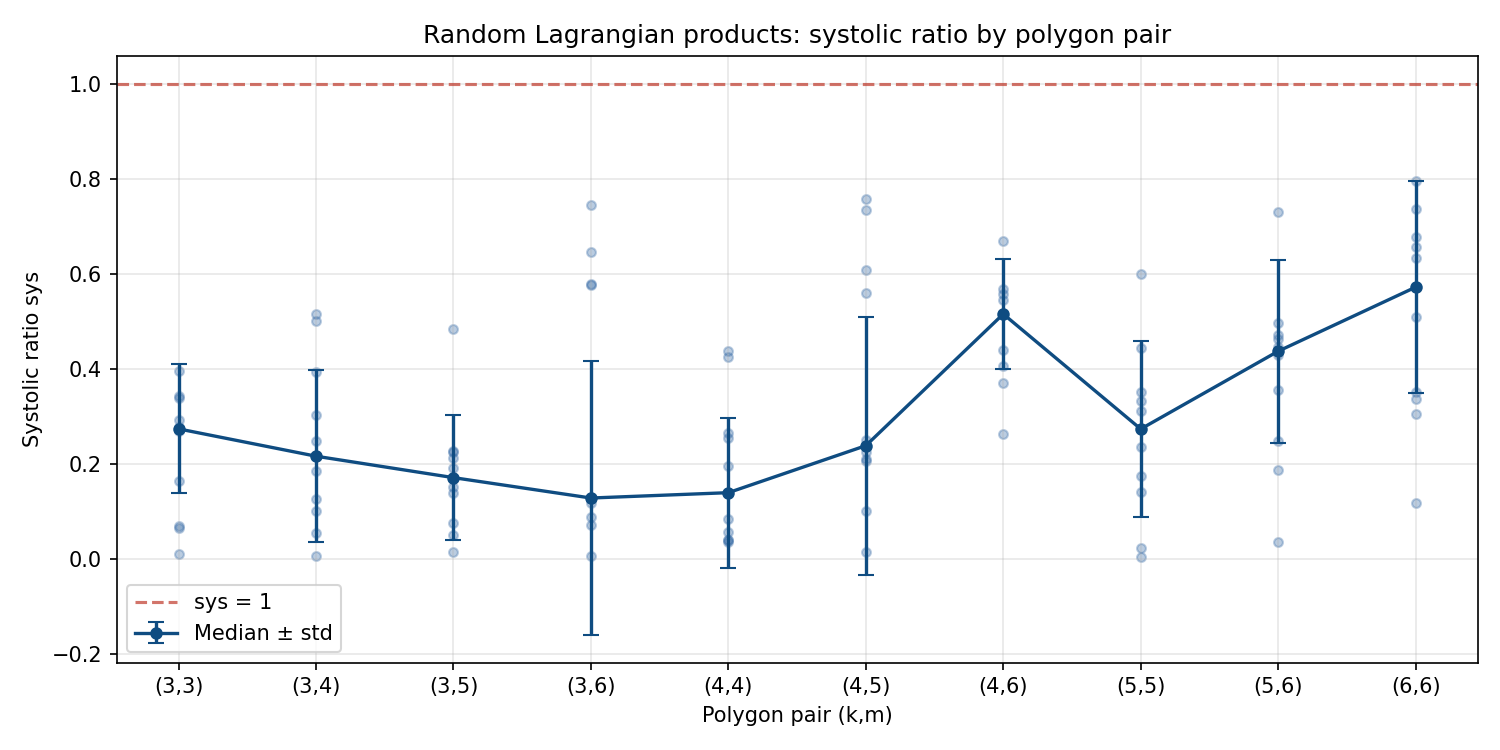
\includegraphics[width=0.9\textwidth]{../experiments/random-product-sweep/random_product_sweep_sys_vs_pair.png}
\caption{Random Lagrangian products: systolic ratio by polygon pair. Each
  bucket corresponds to a polygon pair $(k,m)$ with $3 \le k \le m \le 6$.
  Points show individual samples, and markers with error bars show the median
  and one standard deviation. The dashed line marks $\mathrm{sys}=1$.}
\label{fig:random-product-sweep-sys}
\end{figure}

\subsubsection*{Observations}

No random Lagrangian product exceeds~$\mathrm{sys} = 0.80$, still below
the Viterbo threshold.
The systolic ratio tends to increase with polygon complexity:
$(6,6)$~pairs have the highest median ($0.57$), while
$(3,3)$~pairs have the lowest ($0.27$).

Compared to the random generic sweep
(Section~\ref{sec:random-sweep}, maximum~$\mathrm{sys} = 0.58$),
random Lagrangian products reach higher values
(maximum~$0.79$), suggesting that products are closer to the violation
boundary than generic polytopes.
However, even within the Lagrangian product class, random orientations
do not produce counterexamples.
The known violation ($\mathrm{sys} \approx 1.047$) requires
specific relative rotation angles between the two polygon factors
(Section~\ref{sec:lagrangian-products}), not random orientations---the
rotation parameter is what pushes~$\mathrm{sys}$ above~$1$.
